%
% proposal.tex
%
% Dissertation Proposal Template.
% School of Computing
% Clemson University
%
\documentclass[10pt]{ClemsonProposal}

% This is nice for source code listings
\usepackage{listings}
\usepackage{amsthm}
\usepackage{amsfonts}
\usepackage{amssymb}

\setcounter{secnumdepth}{5}

\newtheorem{thm}{Theorem}

\lstset{
	basicstyle=\footnotesize
}

\lstdefinelanguage{Coq}
	{
		morekeywords={Definition,forall,let,Prop,Function,measure,if,then,else,end,match,with,unfold,intro,elim,reflexivity,replace,simpl,intros,split,change,rewrite,omega,assumption,symmetry,apply,auto,Qed,Theorem},
		sensitive=true,
		morecomment=[l]{--},
	}

\lstdefinelanguage{resolve}
	{
		morekeywords={Definition,Facility,is,realized,by,Var,Concept,uses,Defines,Constraints,Initialization,Type,Family,exemplar,initialization,finalization,ensures,Operation,updates,requires,preserves,clears,evaluates,type,Extension,for,end,if,then,replaces,Procedure,convention,correspondence,iff,extended,Enhancement,Realization,represented,alters,in,modeled,constraint,While,changing,maintaining,decreasing,do,Theorem,For,all,implies,where,and},
		sensitive=true,
		morecomment=[l]{--},
		morecomment=[s]{(*}{*)},
		morestring=[b]",
	}
\lstset{language=resolve}

% This is needed to include figures
\usepackage{graphicx}

% Use any additional packages you might need


%
% Give values to the variables used in this document
%
\title{Engineering Specifications and Mathematics\\for Verified Software}
\department{School of Computing}
\documenttype{Dissertation Proposal}
\major{Computer Science}
\proposalday{8}
\proposalmonth{December}
\proposalyear{2011}
\author{Hampton Smith}
\committeechair{Murali Sitaraman}
\committeememberone{Brian C. Dean}
\committeemembertwo{Jason O. Hallstrom}
\committeememberthree{Roy P. Pargas}

% Just in case you have more then 3 committee members
% \committeememberfour{Member4 Name}
% \committeememberfive{Member5 Name}
% \committeemembersix{Member6 Name}


%
% PDF Setup -- You should not need to change this
%
\hypersetup{
    colorlinks,
    linkcolor={black},
    citecolor={black},
    filecolor={black},
    urlcolor={black},
    pdftitle={\thetitle},
    pdfauthor={\theauthor},
    pdfsubject={\thedocumenttype},
    pdfkeywords={Clemson University, \theauthor, \thedocumenttype},
    pdfstartpage={1}
}


%
% User-specified command definitions/redefinitions
%
\newcommand{\cplusplus}{{\rm C\raise.5ex\hbox{\small ++}}}


\begin{document}
%   ==========================================================================
%   Begin front matter (pages are numbered with roman numerals)
%   ==========================================================================
    \begin{frontmatter}
        \maketitle
		\tableofcontents
        \newpage

        % Generate the abstract
        \chapter*{Abstract}
At the heart of the argument for formal, mathematical methods of software quality assurance is that increased energy spent to develop formal specifications and prove software components against those specifications is amortized over the lifetime of the verified component.  Thus, modularity and reuse are central prerequisites of practical verification.  Because of this, there are two strategies for reducing effective energy invested in a verified component: 1) decrease the amount of effort required to verify it, and 2) increase its reusability and thus its lifetime.

While many modern verification systems exist, few seem to have been designed with modularity and reuse in mind.  On the one hand are systems built on industrial, object-oriented languages, which provide modularity in the programming world, but whose specifications rely on mathematics that do not support these goals.  On the other hand are extensible, generic mathematical systems that are not integrated with programming languages that support component reuse.  The result, on both sides, is the creation of components insufficiently generic and extensible to be reused.

As we wish to verify components of increasing complexity, we must build these components out of smaller subcomponents.  If these subcomponents display poor modularity, they will compose poorly or not at all, resulting in complex interactions and proof obligations that are difficult to satisfy.  To date, modern systems have addressed this complexity by placing the onus of verification on a suite of sophisticated, industrial-strength automated theorem provers that are on the bleeding edge of artificial intelligence design.

This seems paradoxical, however, as programmers do not often rely on deep mathematical results when they reason about the correctness of components.  We posit that by shifting the burden to the design of good components and specifications, as supported by a flexible mathematical and specification subsystem, proof obligations should become much more obvious and more easily-proved.  In addition to influencing the design of our own system, RESOLVE, such exploration would benefit other systems as well, by informing specification and theory design across the board.

This thesis makes three primary contributions.  First, it develops a flexible mathematical framework for program specification designed with modularity and reuse in mind.  Second, presents the design and implementation of a minimalist prover sufficiently flexible to operate on that mathematical framework and determine the actual practical requirements for program verification of well-specified components.  Third, it combines components specified in the mathematical framework with the minimalist verifier to provide evidence in favor of our hypothesis: that well-engineered software should be straightforward to verify.

	\end{frontmatter}



%   ==========================================================================
%   Begin main matter (pages are numbered with arabic numerals)
%   ==========================================================================
    \doublespacing     % Text should be double spaced
    \pagestyle{fancy}  % Turn the nice header on for the rest of the document

\section*{Description of Proposal Area}
\raggedbottom
A verifying compiler ideally eliminates the need for testing to reveal functional bugs by accomplishing what testing cannot: demonstrating the \emph{absence} of any bugs.  Unlike testing and informal reasoning, formal verification demonstrates that code behaves as specified under every possible valuation and along every possible path of execution.

Unfortunately, a number of limitations to full, automatic verification mean that testing remains the norm for quality assurance.  As demonstrated by a number of high-profile software disasters in the past decade, much mission-critical software, upon which human lives may depend, has errors despite rigorous testing.  Only verification can demonstrate that code meets its specification exactly.

Verification operates by viewing code as a series of mathematical transformations and comparing the result with some formal specification of desired behavior.  As a result of this, an important component of any verification system is an automated theorem prover, which takes mathematical statements as its input and attempts to prove them automatically.  However, proving a mathematical statement in general is an undecidable problem and in many modern systems this process must be assisted by a human expert working interactively with the proving system.

Because of the complexity of the problem, these automated provers are on the cutting edge of algorithmic and artificial intelligence design and represent the current bottleneck in automated software verification.  Since mathematical statements are generated from the program's specifications and the specifications are written in the language of the mathematics of the system, the choice of mathematical model has a direct impact on the success or failure of an automated proof attempt.  Often, specifying code one way will yield automatically-verifiable code, while another equivalent specification will not.

The goal of a mechanical verifier has existed since the 1960s and the earliest days of computing\cite{hoareAxiomaticProgramming}.  Despite this, modern verification systems require tremendous effort on the part of highly-trained mathematicians and software specialists to dispatch the proof obligations resulting from even simple programs.  Ameliorating this bottleneck by experimenting with design decision upstream from the prover is the focus of this research.

\pagebreak
\flushbottom
\section*{Explanation of Problem}
A number of open theoretical, practical, and design problems exist in the area of mechanical verification.  Despite a large variety of tools and techniques for verification, a number of these problems span all kinds of systems.  One is the issue of scalability and modularity---to justify the effort required to verify the component, it must enjoy broad reuse so that said effort may be amortized over time.

This research proposes to experiment with factors that contribute to reuse.  We hypothesize that well-engineered, modularly verified code and extensible, reusable mathematics should contribute to more easily verified client systems.  Unfortunately, current verification tools do not generally provide the kinds of tools required to test this hypothesis.  Confirming or rejecting this hypothesis would benefit many existing systems by informing the style of specification used and the choice of where in the verification life-cycle to focus effort to achieve best results.  To successfully explore the problem, a confluence of a flexible mathematical system for specification, an associated prover, and a well-designed library for experimentation is required.

The goal of this dissertation is to experiment with a modularity-focused specification system as well as the consequences of such a design, including the use of a more minimalistic, general automated prover.


    %
    % I use a file for every section.  Each of these corresponds to a file
    % with the specified name ending in '.tex' (e.g., introduction.tex).
    %
    %----------------------------------------------------------------------------
\chapter{Introduction}\label{sect:introduction}
%----------------------------------------------------------------------------
The verifying compiler is a grand challenge in computing, perhaps most famously stated by Tony Hoare in 2003\cite{hoareGrandChallenge}, but based on research into program correctness stretching back to the 1960s\cite{hoareAxiomaticProgramming}.  Such a compiler would ideally eliminate the need for testing to reveal functional bugs by accomplishing what testing cannot: demonstrating the \emph{absence} of any bugs.  Unlike testing and informal reasoning, formal verification demonstrates that code behaves as specified under every possible valuation and along every possible path of execution.

As a powerful demonstration of the weakness of traditional testing and informal reasoning, we consider the case of binary search.  Binary search is a simple, well-understood, and widely-implemented algorithm.  Yet, Joshua Bloch of Google Research wrote a blog post\cite{blochBinarySearch} in 2006 about a subtle bug in the standard Java library's implementation of binary search---an implementation that had been in place for nine years and was based on a version of the algorithm ``proven'' correct (via informal reasoning) by Jon Bentley of Carnegie Melon University in his famous \emph{Programming Pearls}\cite{bentleyProgrammingPearls}.  Certainly, such a straightforward implementation of such a simple algorithm, backed, as it was, by a proof from a respected algorithms guru and in wide deployment for nine years would be considered by most as a \emph{mature}, \emph{well-tested} component---one suitable for use in critical deployments.  And yet it contained a subtle, latent overflow bug revealed not by a nit-picking graduate student but by a client in the wild whose code broke when the component failed to meet its specification (specifically causing an \texttt{ArrayIndexOutOfBoundsException}, which, in a C or \cplusplus context, would be a recipe for a buffer overflow attack in addition to a potential crash.)  This bug, so subtle and resilient against traditional testing and human reasoning, becomes extremely shallow under formal reasoning, where bounded, programmatic integers are well-specified in a mathematical way.

Several systems for formal verification exist, including some built on Java which may have caught this and other bugs.  These systems are traditionally built as a pipeline in which code and its associated specification are translated into an intermediate \emph{assertive code}, which is then translated into a series of \emph{verification conditions} (VCs), which express the proof obligations of the code in a purely mathematical way, before finally being sent to one or more \emph{automated provers} which attempt to dispatch the VCs.  This process is illustrated in Figure \ref{fig:pipeline}.

\begin{figure}
  \centering
    \includegraphics[width=\textwidth]{verification_pipeline}
  \caption{The Verification Pipeline\label{fig:pipeline}}
\end{figure}

Despite many successes, all existing systems require a great deal of effort, either in the form of interactive proving or carefully contrived hints to an automated prover, in order to verify even simple programs.  This is counter-intuitive since most programs contain straight-forward logic that the programmer feels assured of without calling upon complex mathematical reasoning.  The problem is compounded by a lack of integration between between modern, modular programming languages and expressive, flexible mathematics that prevents the design of reusable components, which could amortize this intense verification effort over time.  We hypothesize that a well-integrated, flexible and extensible mathematical and specification subsystem would permit specifications that more closely reflect the programer's intuition and the usual patterns of reuse, resulting both in more straightforward proofs and more generic, longer-lived components.  This proposal seeks to develop such a system and test this hypothesis.

%----------------------------------------------------------------------------
\section{Existing Systems: Practical vs. Pure}
%----------------------------------------------------------------------------
Existing verification systems largely fall into two categories: those with a focus on practical, automated verification and those with a focus on pure mathematics.  Examples of the former include Jahob\cite{kuncakJahobOverview}, based on Java; Spec\#\cite{specsharp}, based on C\#; and ACL2\cite{kaufmannACL2}, based on Lisp.  Examples of the latter include Coq\cite{coq}, based on the Calculus of Inductive Constructions; and Isabelle\cite{nipkowIsabelle}, based on a higher-order, intuitionistic logic.  Practical systems often take advantage of a limited, hardcoded mathematical universe that corresponds closely to or is conflated entirely with programming constructs.  Pure systems permit an extensible, flexible mathematical framework with clear separation of programming concepts from mathematics.  Because of their narrower focus, the former often permit easier mechanical verification than the latter\footnote{Some systems even permit efficient decidable verification algorithms for certain domains or properties.  See, e.g., information on SplitDecision in \cite{Sit11}.}, which tend to emphasize interactive user-guided verification.

%----------------------------------------------------------------------------
\subsection{Example Practical System: Jahob\label{sec:exPractical}}
%----------------------------------------------------------------------------
Let's consider a version of Java's \texttt{ArrayList} verified in Jahob\footnote{Jahob does not yet work with Java generics and so the version of ArrayList verified is the pre-Java-1.5 version that operates on \texttt{Object}s.}.  Jahob combines code written in a subset of Java with specifications written in Isabelle.  Listing \ref{lst:alcontains} shows the \texttt{contains()} operation of an ArrayList.

\lstinputlisting[language=Java,caption={ArrayList.contains()\label{lst:alcontains}}]{ArrayList1.java}

The list is modeled as a set of $(index, element)$ pairs.  Assertions are provided inside Java comments (meaning that Jahob-specified Java programs remain compilable using a standard Java compiler) that begin with a colon.  Note that mathematical assertions are set off in quotes, a syntax inherited from Isabelle.  \texttt{init} is a predicate defined elsewhere in the class.  Jahob encourages the inclusion of inline ``hints'' targeted at the backend provers\cite{zeeIntegratedProofLanguage} (of which it supports many) and we see several of those here interspersed in the Java code.

Utilizing a suite of provers, the Jahob system is able to dispatch the resultant VCs and yield a fully-verified \texttt{ArrayList} implementation suitable for generic use---an impressive feat.  In fact, in a recent result, the Jahob team verified a handful of different linked data structures\cite{zee:annotations}.  A number of design decisions support this ability.  First, Jahob has a flexible set of syntactic tools for specification, including pre- and post- conditions, auxiliary variables\cite{kingVerifier}, and conceptual definitions that permit an intuitive specification.  Second, while Jahob supports higher-order specifications, where possible it uses a standard first-order logical representation that can be translated into the input format of multiple back-end proving systems including CVC3\cite{barretCVC3} and Z3\cite{deMouraZ3}.  Those specifications that cannot be translated down to a first-order representation can still be sent to Isabelle for interactive proving.  By using multiple prover backends, Jahob can take advantage of multiple proving paradigms including interactive, algebraic, boolean satisfiability (SAT) solvers, and efficient decision procedures.  Third, as already stated, Jahob permits in-line mathematical assertions that allow the programmer to guide backend provers by stating useful intermediate results.

However, despite this success, a number of the realities of this system (and others like it) are counter-intuitive and seem geared toward short-term verification of small Java programs rather than long-term, scalable verification of complex, modular applications.

\paragraph{Complex Proof Obligations for Simple Methods.\label{sec:jahobComplexVCs}}
When using the Jahob system, VCs that result from even simple programs are often extremely complex. Jahob's intermediate VC syntax is not intended to be human readable, so we do not reproduce any VCs here, but we can get a feel for their complexity via sheer volume: the three-line boolean method \texttt{contains()} generates VCs that span over 150 lines\footnote{When formatted to standard 80-character lines.}.  

A number of factors contribute to this VC complexity.  First, Jahob is built on top of an existing programming language that includes many features that are not amenable to verification, including null pointers and uncontrolled aliasing, both of which complicate reasoning\cite{weideVerificationReferences}.  These complexities must be accounted for in its VCs.  Second, Jahob's inline assertions must themselves be verified to preserve soundness.  The intent of these assertions is that they simplify the proving process by proving intermediate steps, creating additional (presumably easier) VCs that in turn lower the difficulty of the original proof obligations.  Still, why intermediate results should be required for a simple \texttt{contains()} method is unclear.  Third, while perhaps subjective, the system encourages the use of awkward mathematical models for components.  In the list example, the choice of a set for mathematical model requires additional invariants to establish that, for example, no index in the list appears twice with different elements.  Presumably a set was chosen because it was the closest mathematical object that already had a well-developed Isabelle theory, but in an ideal world such a system would provide a first-class, integrated mechanism for extending the mathematical universe so that a more directly analogous mathematical object could be used---perhaps a function mapping or a finite sequence abstraction.

\paragraph{Lack of Support for Modular Design.\label{sec:jahobNoModularity}}
Jahob stands nearly alone amongst the practical systems for supporting higher-order mathematics.  However, practical issues with the integration of Isabelle into Java hamstring the usefulness of this feature.  Among the Java features not supported by Jahob are Java generics and dynamic dispatch.  These unsupported features preclude many important patterns of reuse that the mathematics of Isabelle are otherwise ready to support.  Components cannot be parameterized from the outside with definitions (this is not supported directly and programmatic work-arounds like the Strategy and the Template design patterns rely on dynamic dispatch.)  Data structures cannot make parameterizable guarantees about the properties of contained elements (which would require Java generics.)  Indeed, the majority of the polymorphism pillar of object-orientation is precluded, seriously reducing the reusability of components and thus the amortization of verification effort over time.

A particularly illustrative example of this lack of modularity appears in a \texttt{Map} data structure verified by the Jahob team in \cite{zee:annotations}.  The trouble of aliased keys is dealt with by specifying that \emph{all objects} are immutable with respect to the built in Java \texttt{hashcode()} method---a restriction that does not appear in the original \texttt{Object} contract and further implies that all objects are immutable with respect to \texttt{equals()}.  The correctness of the \texttt{Map} implementation requires changes to external components, rather than being part of its self-contained specification.  We discuss this problem in more detail in \cite{bronishMap}.

\vspace{1.5em}With lengthy, complex VCs, syntax for guiding back-end provers, and a system that encourages a trade-off of mathematical flexibility for prover diversity, the Jahob design seems to assume that the onus of verification is on the provers.  It shifts the complexity of verification to the part of the pipeline highlighted in Figure \ref{fig:prover}.  However, as the strength of automated provers is the current bottleneck of verification, this requires a great many sacrifices to the limitations of this bleeding-edge part of the verification toolchain.

\begin{figure}
  \centering
    \includegraphics[width=\textwidth]{proverpart}
  \caption{Shifting the Burden to the Prover\label{fig:prover}}
\end{figure}

%----------------------------------------------------------------------------
\subsection{Example Pure System: Coq\label{sec:exPure}}
%----------------------------------------------------------------------------
Let's consider a recursive implementation of the integer division operator, specified and implemented in Coq.  Despite the fact that Coq is a mathematical system, unable to execute code, we could use its ability to ``extract'' a program into various target languages\footnote{At time of writing: OCaml, Haskell, and Scheme.} for execution.  Coq separates specification from implementation; in Listing \ref{lst:divpred} we see a pair of predicates for specifying integer division.

\lstinputlisting[language=Coq,caption={Division Predicates\label{lst:divpred}}]{DivPred.coq}

The \texttt{divPre} predicate represents the precondition on division---that the second argument is not 0.  The \texttt{divRel} predicate specifies the relational behavior of division---that the result will consist of two natural numbers, \texttt{q} and \texttt{r}, such that \texttt{q * d + r = n} and \texttt{r < d}, i.e., \texttt{q} is the quotient and \texttt{r} the remainder.

We then implement division recursively as shown in Listing \ref{lst:divimpl}.

\lstinputlisting[language=Coq,caption={Division Implementation\label{lst:divimpl}}]{DivImpl.coq}

Coq's \texttt{Function} keyword introduces a recursive function with an appropriate implicit fixpoint.  The \texttt{measure} keyword provides a progress metric---namely, that \texttt{fst} is decreasing.  Note that, despite the fact that an input matching \texttt{(\_,0)} is disallowed by the precondition, Coq does not permit non-total functions, so we provide a nonsense return value for this case.  The \texttt{le\_lt\_dec} is simply a less-than-or-equal-to predicate on natural numbers. Defining this function immediately raises a termination proof obligation, which one of Coq's built-in proof scripts can dispatch automatically.

To demonstrate the correctness of the implementation, we can assert the theorem given in Listing \ref{lst:divtheorem}.  That is, that for all inputs, if the inputs meet the precondition, then the behavioral relation holds between the inputs and the result of applying \texttt{div}.

\lstinputlisting[language=Coq,caption={Division Functional Correctness Theorem\label{lst:divtheorem}}]{DivTheorem.coq}

Proving this theorem is more complicated than the termination proof and none of Coq's built-in tactics can dispatch it automatically.  Instead we enter interactive mode and prove it live with the sequence of tactics given in Listing \ref{lst:divproof}.

\lstinputlisting[language=Coq,caption={Division Functional Correctness Proof\label{lst:divproof}}]{DivProof.coq}

A high-level sketch of this proof is that it applies induction by cases, proving that each of the \texttt{match} branches and each of the \texttt{if} branches maintains the correctness of the implementation.  Definitions are repeatedly expanded to take advantage of their hypotheses.  Obviously, however, this syntax is far from readable without being intimately familiar with Coq and certainly looks nothing like a mathematical proof as it might be conceived by a mathematician.

Systems like this have been used to excellent effect verifying complex programs.  Coq has been used to verify a C compiler\cite{leroyVerifiedcompiler}, while Isabelle has been used to verify an operating system kernel\cite {kleinVerifiedOS}.

This success is due to a number of factors.  Unlike in the practical programming systems, Coq and other pure systems provide a rich, extensible mathematical universe permitting higher-order logic and user-created mathematical theories.  This enables a hierarchy of abstraction similar to the development of object oriented code in which complex mathematical objects are repeatedly decomposed into smaller and smaller mathematical objects and an ``interface'' of theorems is provided for working with the high level objects.  In addition, Coq's programming model is functional, eschewing a number of complexities pervasive in industrial languages---pointers, aliasing, and referential opacity to name a few.  Automated proof systems are used to jump small steps, but interactive mechanisms are provided for splitting complex proof obligations into multiple smaller tasks.  It's as though the human user becomes part of the assertive code and VC generation step, pointing out useful decompositions of existing proof obligations until they become small enough that the automated prover can take it from there.  In a sense, such a system shifts the onus of the verification process to the part highlighted in Figure \ref{fig:assertivecode}.

\begin{figure}
  \centering
    \includegraphics[width=\textwidth]{vcpart}
  \caption{Shifting the Burden to the VC Generator\label{fig:assertivecode}}
\end{figure}

Unfortunately, given the value of a highly-trained mathematical and programming professional's time, a user-guided strategy is likely cost-prohibitive if all but the smallest proof obligations must be discharged by hand.  A number of factors contribute to the difficulty of these proof obligations.

One is that, in order to exploit the flexibility of the mathematical system, the automated prover must be more general, unable to take advantage of the numerous domain-specific tricks that cutting-edge narrowly-applicable theorem provers exploit.  Another is that the divide between the mathematical world of Coq and the programming world of an industrial language is large.  We see an example of this in the division example, where time and effort must be expended proving that the behavioral relation is total (even though the method it specifies is not!) and that an irrelevant program branch maintains invariants.

Compounding this problem, pure systems have no awareness of the underlying programmatic structure they are being applied to and thus inherently view verification as operating on procedural rather than object-oriented code.  Modular mathematics are therefore not applied to modular code and the result is that, impressive as a verified compiler is, the next complex component must be verified from scratch as it is unlikely that any component from the compiler will be generic enough to be reusable.

%----------------------------------------------------------------------------
\section{Best of Both Worlds?}
%----------------------------------------------------------------------------
At the core of this research is the question of whether or not a system that combines the best parts of practical systems and the best parts of pure systems might permit specifications that are more amenable to automatic verification.  A programming system that eschews certain complexities of industrial languages and avails itself of a tightly-integrated, flexible and extensible mathematical system designed to work with it could be used to create modular components based on modular mathematics.  We hypothesize that in such a system, a focus on modularly verified components would yield less complex proof obligations while at the same time encouraging the creation of reusable components that amortize the verification effort invested in them over time.  Such a system would place the onus of the verification on the design of modular specifications supported by a flexible compiler, i.e., that part of the pipeline highlighted in Figure \ref{fig:specification}.  Highly trained programmers and mathematicians are still required, but the fruits of their labors will be generic and reusable, unlike proofs of correctness.

\begin{figure}
  \centering
    \includegraphics[width=\textwidth]{specpart}
  \caption{Shifting the Burden to Specification\label{fig:specification}}
\end{figure}

Developments such as these would also benefit existing systems of all types.  Increased understanding of the importance and techniques of modular reasoning can be applied to systems like Jahob to increase the provability of large components via better-engineered subcomponents.  A richer understanding of the importance of levels of mathematical abstraction to long-term verification goals would assist those working in pure system like Coq in making better up-front choices to pay long-term dividends.

%----------------------------------------------------------------------------
\section{Problem Statement}
%----------------------------------------------------------------------------
This proposal seeks to determine if the mechanical verifiability of software components can be improved by better-engineered mathematics and specifications and, if so, explore which techniques might best support these goals.  In the process it will address the following open problems in the area of formal methods:

\begin{itemize}
\item Design of an extensible, flexible mathematical framework and a well-integrated associated specification framework, supporting verifiability by allowing specifications based on the \emph{best} mathematical model, rather than simply the most convenient, and supporting scalability through mathematical reuse.
\item Architecture of and experimentation with a minimalist rewrite prover to support reasoning in the above framework and determine those prover capabilities practically necessary to mechanically verify well-engineered, modular components.
\item Creation of a diverse library of components of the sort found in standard programming libraries, specified and modeled using a broad set of techniques to enable experimentation on mathematical and specification best-practices for practical verification.
\end{itemize}

%----------------------------------------------------------------------------
\section{Research Approach}
%----------------------------------------------------------------------------
Building on previous work on specification language design, VC generation, and automated prover development, this research seeks to augment the existing RESOLVE\cite{Sit11} system with a flexible mathematical subsystem and modular specification subsystem in order to experiment with the specification and mathematics best-practices in support of modularity.

Unlike practical systems, where bringing modular mathematics to bear in support of modular programming is difficult at best and where special-case constructs like references cause complex reasoning even in situations where they ought not be relevant, the mathematical system proposed here will be tightly integrated and based on an extensible Morse-Kelley Set Theory, extended to include higher-order definitions, and will permit specification of programmatic constructs (e.g., references) only as modeled in that pure mathematical system.

Unlike pure systems, where the specification system that bridges between mathematics and programming is ad-hoc and not designed to take advantage of the structure of a program, the specification system proposed here will cooperate with the mathematical system by design, thus permitting it to take advantage of the same modularity and genericity used in a well-designed component.

Armed with such a system, we will test its flexibility by designing, specifying, and implementing a library of programming components ranging from simple stacks to more complicated tree structures, along with the algorithms for manipulating these structures.  These structures and algorithms will be modeled and specified using a variety of techniques in order to gain insight into how these techniques impact verifiability and scalability.  We will analyze resulting VCs to determine which prover capabilities are strictly necessary, designing and building a minimalist rewrite-based prover based on a plug-in architecture to support only those capabilites necessary for practical VCs.

The evaluation of the system as a whole will include classification of VCs by the minimalist prover based on a number of proof metrics including number of required theorems, number of required proof steps, and proof time; as well as subjective, qualitative metrics derived from field tests with programming and mathematics students and professionals.

%----------------------------------------------------------------------------
\subsection{Contributions\label{sec:contributions}}
%----------------------------------------------------------------------------
Such a system would address several open problems in the area of formal methods, both practical and theoretical:

First, a flexible, extensible, and intuitive mathematical subsystem would significantly improve on a key component of the verification tool chain.  The day when an AI can infer the intent of a program and verify it without rigorous specification and significant mathematical development is extremely distant.  Until that time, formal verification will be a joint effort between highly trained programmers and mathematicians.  While improvements are being made\cite{wenzelIsar}, the current generation of specification systems (both practical and pure) largely use ad-hoc mathematical syntax and esoteric mathematical foundations that programmers may find convenient but mathematicians find confusing and unweildy.  Beyond simply engendering collaboration between programmers and mathematicians, such a math-centered language design will encourage the full body of modern mathematical developments to be used directly.  Additionally, since it is not grounded in any programming constructs, it will not be tied to any particular language and may itself be used as a component outside of RESOLVE.

Second, a well-integrated and flexible specification and mathematical system would open up the development of verified components to modular, reusable techniques by providing first-class syntax and flexible mathematical semantics for mapping such programmatic ideas into the mathematical realm.  As an example, the lack of useful higher-order logic in practical systems prevents components from being designed to take mathematical assertions or abstract operations as parameters, severely limiting one dimension of reuse: genericity\cite{bronishMap}.  Our hypothesis is that a well designed, modular system should better exploit programmer intuition and allow for more straightforward proof obligations, permitting slower, but more expressive, automated provers to be used.  The development of such techniques would be a boon to existing systems, as well.  For example, as part of our research so far, we have explored the concept of quantifier elimination and techniques that can be used to specify and verify in their absence.  In a recent paper from the Jahob team, we find a quote highlighting the need for such research, here in the context of an attempt to verify an implementation of a Java \texttt{ArrayList}: ``Unfortunately, the provers are unable to automatically prove the post-condition of remove.  What makes the problem...difficult is that the assumptions contain universally quantified formulas while the post-condition contains an existentially quantified formula.''  Our research on engineering mathematics addresses this and other issues and may be helpful in elliminating such complications.

Thirdly, such a system will permit the above hypothesis to be tested and demonstrated in a rigorous, mechanical environment.  The current state of the art in verification suggests that verification is hard because programs are complicated.  We believe that well-engineered programs are not complicated and that, by extension, if augmented with well-engineered specifications, the resulting proof obligations should not be difficult.  Thus, a system designed to support well-designed programs is more important to successful verification than one designed to support the limitations of a state-of-the-art prover.  What such a design entails and what it means to be a ``well-engineered specification'' are open questions addressed by this research.

%----------------------------------------------------------------------------
\section{Thesis Statement}
%----------------------------------------------------------------------------
In a verification system, an extensible, flexible mathematics and specification subsystem enables better-engineered component specifications and thus more straightforward proof obligations that are more easily dispatched by even minimalistic automated theorem provers.

%----------------------------------------------------------------------------
\section{Proposal Organization}
%----------------------------------------------------------------------------
The remainder of this proposal is organized as follows: Section~\ref{sec:background} gives an overview of the state-of-the-art in each of the problem areas, with information on work related to this research, Section~\ref{sec:resolveBackground} provides background on the RESOLVE verification system that is the platform for this research, Section~\ref{sec:research} presents the proposed research including work already completed, Section~\ref{sec:evaluation} explains the criteria against which the work will be evaluated, and Section~\ref{sec:conclusion} will offer some concluding thoughts.

    \include{background}
    %----------------------------------------------------------------------------
\section{RESOLVE Background}\label{sec:resolveBackground}
%----------------------------------------------------------------------------
The RESOLVE\cite{RESOLVE} Verifying Compiler is an attempt to create a full verificatin pipeline, beginning with an integrated specification and programming language and continuing through to a back-end prover.  The focus of RESOLVE is on modular verification, which attempts scalability by ensuring that each component is verified in isolation and need not be re-verified regardless of deployment.  This means that encapsulation must be strictly assured and thus certain treacherous programmatic constructs such as aliases must be tightly controlled.

As an example, let's consider a Stack abstraction.  We are interested in designing a system for complete verification---including constraints like memory, so we will use a bounded stack that takes as a parameter its maximum depth.  Listing \ref{lst:stack} shows part of a RESOLVE concept describing such a component.

\lstinputlisting[language=resolve,caption={A Stack Concept\label{lst:stack}}]{Stack_Template.co}

RESOLVE permits parameterized types.  In this case \texttt{Entry} is a generic type, permitting \texttt{Stack}s to operate over any other RESOLVE type, and \texttt{Max\_Depth} is an integer indicating the maximum number of elements that can ever be on the stack.  The \texttt{evaluates} parameter mode indicates that the parameter is pass-by-value (parameters are ordinarily pass-by-reference.)

Applying modular lessons from the world of programming to mathematics, we store theories in separate files with their own scopes that can be imported individually\cite{smith08}.  The \emph{uses} line includes one such file---the theory of strings, i.e., finite sequences.

The \texttt{Family} clause introduces a family of abstract types called \texttt{Stack}s, modeled conceptually by strings of \texttt{Entry}s.  \texttt{exemplar} introduces a name to be used for a hypothetical stack, which is then used in the \texttt{constraint} clause to indicate that not \emph{all} strings of \texttt{Entry}s are valid stacks, but rather only those of length \texttt{Max\_Depth} and less.  The \texttt{initialization} clause notes that all \texttt{Stack}s are assured to be empty when they are first created.

We then define some operations on \texttt{Stack}s---\texttt{Push()} and \texttt{Pop()}, with their associated pre- and post-conditions, introduced by \texttt{requires} and \texttt{ensures} clauses, respectively.  Parameters to operations are preceded by \emph{parameter passing modes}, which summarize the effect the operation will have on a parameter---a parameter that's in \texttt{alters} mode is passed a meaningful value that will be changed to an arbitrary value by the end of the call; an \texttt{updates} parameter is given a meaningful value that will be changed to a new meaningful value as specified in the \texttt{ensures} clause;  a \texttt{replaces} parameter will be passed an arbitrary value and be changed to a meaningful value by the end of the call.

\texttt{requires} and \texttt{ensures} clauses are mathematical assertions and their variables refer to the mathematical models of the parameters.  So, while \texttt{Push} operates on physical \texttt{Stack}s, \texttt{S} in its \texttt{ensures} clause refers to the mathematical representation of the passed stack---a string of \texttt{Entry}s.  Because mathematical variables can have only one, unchanging value, we use the pound sign to indicate the value at the beginning of the call.  Thus, \texttt{\#S} refers to the value of the \texttt{Stack} at the beginning of the call and \texttt{S} refers to its value at the end.  Inside a \texttt{requires} clause there is no conception of the the values of parameters at the end of the call and so pounds are not used and all variables refer to the values of parameters at the beginning of the call.

Angled braces and the \texttt{o} operator come from \texttt{String\_Theory} and represent the singleton-string constructor and the concatenation operator respectively.

Once a concept has been described, an implementation can be provided in a \emph{realization}.  Listing \ref{lst:linkingrealization} provides a realization of a \texttt{Stack} using an array.  Note that while we provide some syntactic sugar for arrays, a pre-processing step translates all array manipulation into interactions with a normal component and thus all reasoning is accomplished via a specification that models arrays as functions from integers to entries rather than hard-coded or specialized array reasoning.  This contrasts with every other practical programming verification system we are aware of that supports arrays and provides an example of how often-primitive structures can be modelled normally within the framework of RESOLVE's flexible mathematical subsystem\footnote{In addition to this array-based implementation, we are experimenting with a linked-structure mathematical component in order to provide, in this case, a linked-list based implementation.  The details of this exploration can be found in \cite{kulczyckiPointers}.}.

\lstinputlisting[language=resolve,caption={An Array Realization\label{lst:linkingrealization}}]{Array_Realiz.rb}

We represent our Stack programmatically as a \emph{record} (similar to a \emph{struct} in C) containing an array of contents and a top index.  A \texttt{convention} represents an \emph{invariant} that must hold after initialization, before finalization, and before and after each method.  In this case, the top must be at a valid index (save index 0, where it is permitted to reside if the Stack is empty.)

A \texttt{correspondence} provides a mapping between the physical \texttt{Stack} and its mathematical conceptualization, in this case using a mathematical definition \texttt{Concatenation}, which is to string concatenation what big $\Sigma$ is to integer addition, to build a string of all its elements.

A procedure is provided for accomplishing both \texttt{Push()} and \texttt{Pop()}, taking advantage of standard integer and array operations.

Using the specifications of these operations, the RESOLVE compiler is able to generate VCs establishing the correctness of this \texttt{Stack} implementation.  The details of this generation process is the topic of \cite{hartonDissertation}.  As an example, this is the VC establishing the convention at the end of a call to \texttt{Push()}:

\lstinputlisting[language=resolve]{Pop_Convention.asrt}

Note that in Given \#10, the length of the result of the concatenation is clearly equal to \texttt{S.Top}, thus we know that \texttt{S.Top + 1} is less than \texttt{Max\_Depth}, satisfying half the goal.  Then, by Given \#9, we see that \texttt{0 <= S.Top}, so clearly \texttt{0 <= (S.Top + 1)}, satisfying the other half.

Once generated, VCs are passed to RESOLVE's integrated minimalist prover.  This prover was built as an extensible prover platform for verification experimentation\cite{smith10} and is discussed more thoroughly in Section \ref{sec:researchProver}.

Concepts may further define \emph{extension operations}, which are secondary operations describing useful operations that not all realizations will be able to implement practically or efficiently.  As an example, \texttt{Stack\_Template} has an extension operation called \texttt{Flip}:

\mbox{\lstinputlisting[language=resolve]{Flipping_Capability.en}}

Just as with a concept, enhancements may have multiple associated realizations, for which the VC-generation and proving process is the same.  Consider the realization of \texttt{Flipping\_Capability} given in Listing \ref{lst:flipRealiz}.

\lstinputlisting[language=resolve,caption={A Realization of Flip\label{lst:flipRealiz}}]{Obvious_Flip_Realiz.rb}

This flipping procedure establishes a new \texttt{Stack}, \texttt{S\_Flipped}, then iteratively pops each element off the original stack and into the new one.  Having done so, the \texttt{:=:} operator swaps the value of \texttt{S\_Flipped} with \texttt{S}.  Using swapping as its basic data movement operator enables RESOLVE to minimize undesirable aliasing\cite{harmsSwapping}.

Notice that the while loop requires a number of annotations.  The \emph{changing} clause establishes a frame property: only those values explicitly listed may change.  The \emph{maintaining} clause establishes a loop invariant expressing the logic of the loop.  Finally, the \emph{decreasing} clause establishes a termination metric to allow us to guarantee termination.

Such annotations are standard operating procedure for verification systems and can be seen across the board at, for example, the first VSTTE verification competition\cite{klebanovVSTTEExperience}.  We note, however, that some work has been done on automatically discovering, e.g., loop invariants on the programmer's behalf\cite{ernstInfer}.  RESOLVE's explicit invariants do not preclude such a method from being employed to fill them in.

Using RESOLVE's integrated minimalist prover, a component of this research, we are able to fully and mechanically verify this procedure, as will be discussed further in Section \ref{sec:research}.

    %-----------------------------------------------------------------------------
\chapter{Research}\label{sec:research}
%-----------------------------------------------------------------------------
In this document, we have proposed to design a new mathematical and specification subsystem for a mechanical verifier, experiment with the capabilities of a minimalist prover, and apply these to determine the efficacy of specification and mathematical engineering techniques over a library of verified components.

The design of this system will be based on our experience writing and verifying reusable components using the existing RESOLVE verifying compiler, as well as applying lessons from our previous research.

Work on the research proposed in this document will proceed along the path outlined in the introduction, addressing the three points of the problem statement directly in order to test our thesis.

%-----------------------------------------------------------------------------
\section{Extensible, Flexible Mathematics for Specification}
%-----------------------------------------------------------------------------
Because every component that is to be verified must be modeled mathematically, the expressiveness of the mathematical system has a direct impact on the facility of the modeling process.  By extension, this impacts the facility of the specification of operations as well, as they must necessarily operate on these mathematical models.  In order to permit components to be modeled and reasoned about at the best level of mathematical abstraction, rather than simply the most convenient, a verification system must permit an extensible mathematical language.  In order to promote the amortization of verification effort over time, the mathematical language must be flexible enough to support patterns of reuse.

Most practical systems do not meet these goals, as their mathematics are limited or built in.  Many pure systems meet them in the mathematical realm, but fail to support the levels of integration with the programmatic realm required to reap the anticipated benefits.  We propose to address this by combining an extensible, flexible mathematical system like those found in pure languages with the modular, reusable techniques of a modern object-based language like those expected for practical systems.

%-----------------------------------------------------------------------------
\subsection{Work Completed}
%-----------------------------------------------------------------------------
As we have already published in \cite{bronishMap}, genericity and modularity are crucial attributes of a useful verified component (in that paper, a Map data structure) and systems with inflexible mathematics often sacrifice these attributes by focussing on verifiability alone, yielding verified, but not terribly useful, components.  The mathematical and specification subsystems of our current RESOLVE prototype already contain many features that exemplify the sort of mathematics for verification that we propose.  However, further work is needed to make them extensible and intuitive and to increase the robustness of the implementation.  After much experimentation, described in the various \emph{Work Completed} sections, we have identified the current type system as a major weakness and barrier to extensible, flexible design.  In conjunction with mathematicians here at Clemson and at Ohio State, we have designed a new type system that will be more flexible, more closely match a modern mathematician's conception of the mathematical universe, and, at the same time, be easier to implement because of its regular and reflective nature.

Our new design exploits four key design principles to permit an extensible, flexible system:

%----------------------------------
\subsubsection{Higher-Order Logic.}\label{sec:higherOrderDefinitions}
%----------------------------------
If our verified components are to be worth the time we spend verifying them, they must be suitably generic to ensure broad reuse.  Many reuse patterns found in modern programming languages are difficult or impossible to specify or verify using the first-order logic dictated by most practical verification systems and automated provers.  In particular, they make it difficult to apply the lessons of programming to the mathematical world.

Consider, for example the $foldr$ function ubiquitous in functional languages.  $foldr$ takes as its parameters a starting value of type $\gamma$, a function of type $(\gamma*\delta)\rightarrow\gamma$, and a list of elements of type $\delta$.  Starting with the starting value and the first element of the list, the function is applied to yield a new value of type $\gamma$ before repeating the procedure with the resultant value and the next element of the list.  The result of the final function application is returned.  A summing function for lists of integers could thus be defined as:

$sum(zs) = foldr(0, +, zs)$

The broad applicability of such a function for specification should be obvious.  However, even simple theorems describing the mathematical properties of this function run afoul of the first-order restriction that functions may not be quantified over.  For example, Theorem \ref{thm:emptylist} states that $foldr$ applied with an initial value to an empty list simply returns the initial value:

\begin{thm}
$\forall f : (\gamma*\delta)\rightarrow\gamma, \forall ds : List(\delta), (|ds| = 0) \Rightarrow (foldr(i : \gamma, f, ds) = i)$
\label{thm:emptylist}
\end{thm}

Creating definitions that operate on functions is similarly curtailed, preventing development of reusable theories of, for example, transitive functions.

Because our minimalist prover leaves functions and definitions \emph{uninterpretted}, quantifying over them becomes straightforward.  A function or definition is uninterpretted when we do not expand it to consider its definition---i.e., the mathematical subsystem looks at a function or definition variable as a black box, treating it no differently from an ordinary variable.  The tradeoffs inherent in such a design decision are discussed more completely in \cite{tagoreExpand}.

%----------------------------------
\subsubsection{First-class Types.}\label{sec:firstClassTypes}
%----------------------------------
First-class types are a feature of several mathematical systems and a handful of experimental programming languages, but were not a part of the original RESOLVE design.  The current prototype treats types as a special case, which makes them difficult and inconsistent to manipulate, limiting the facility of mathematical extension.

The new design incorporates first-class types that are treated as normal mathematical values.  They can be manipulated, passed as parameters, returned as the result of a relation, and quantified over.  This provides both a great deal of flexibilty, as well as a straightforward mechanic for specifying certain generic programming paradigms (most obviously: parameterized type variables.)

For example, the following line would introduce a particular integer called \textbf{1}:

\begin{lstlisting}
Definition 1 : Z = succ(0);
\end{lstlisting}

In exactly the same way, a new type called \textbf{N} could be defined:

\begin{lstlisting}
Definition N : Power(Z) = {n : Z | n >= 0};
\end{lstlisting}

The symbol table maintains information about the kinds of elements that make up any existing class and can thus infer when the symbol introduced by a definition can safely be used as a type.  Thus this is a valid sequence of definitions:

\begin{lstlisting}
Definition N : Power(Z) = {n : Z | n >= 0};
Definition NAcceptor(m : N) : B = true;
\end{lstlisting}

But this one is not:

\begin{lstlisting}
Definition 1 : Z = succ(0);
Definition OneAcceptor(o : 1) : B = true;
\end{lstlisting}

Note that the ``type'' \texttt{Power(Z)} is not actually a type, but rather a function that takes one type and returns another--itself an example of first-class types in action.

Type schemas and dependent types, which define generalized types parameterized by other values, also take advantage of the first-class nature of types and can be defined as normal relations that return a type, rather than using a special syntax.  This requires values that are, in some sense, \emph{of type Type}.  We call this type \textbf{MType} as an abbreviation for \emph{Math Type}\footnote{\texttt{MType} is comparable to * in Haskell, where * is the kind of a type.}.

\begin{sloppypar}
So, as a complete example, consider the String type schema, which represents a finite sequence of elements of a certain type, presupposing the existence of a type \textbf{UntypedStr}, which contains all finite sequences of elements of possibly heterogenous type, and a function called \texttt{Contains\_Only\_Elements\_Of\_Type()} which returns \texttt{true} if and only if a given UntypedStr contains only element of the given type:
\end{sloppypar}

\begin{lstlisting}
Definition Str(T : MType) : MType = 
	{S : UntypedStr | Contains_Only_Elements_Of_Type(S, T)};
\end{lstlisting}

Because they are treated like any other values, such first-class types can be reasoned about by all the same mechanisms already in place for other mathematical values.

%----------------------------------
\subsubsection{Mechanisms for Static Reasoning.}\label{sec:staticreasoning}
%----------------------------------
A practical problem with first-class types is the ability to specify types and type-matching situations that are undecidable.  This is an issue common to all systems that permit dependent types--which a system of truly first-class types must necessarily do.

For example we could imagine two types defined by arbitrary predicates:

\begin{lstlisting}
Definition T1 : MType = {E : MType | P(E)};
Definition T2 : MType = {E : MType | Q(E)};
\end{lstlisting}

Determining whether or not an object modeled by \texttt{T1} can be passed where one modeled by \texttt{T2} is expected is equivalent to asking if $\forall e : $\texttt{MType}$, Q(e) \rightarrow P(e)$, which is, of course, undecidable.

Some verification systems (e.g., Coq) take advantage of this very property as an aid to verification, reducing all programs to reasoning about complex types and casting verification as a type-matching problems.  However, because our goal is to permit the use of flexible mathematics on top of a foundation that takes advantage of standard programming models, we would ideally like to provide the usual static type-safety expected by object-oriented programmers.

To this end, we will largely refuse to attempt matching arbitrary mathematical types, relying instead on the programmer or mathematician to provide an explicit mapping in cases where the reasoning is complicated.

In some cases, relationships can be easily inferred.  For example, the case of simple sub-types:

\begin{lstlisting}
Definition Z : MType = ...;
Definition N : Power(Z) = ...;
\end{lstlisting}

Here we can easily note in the symbol table that an \texttt{N} would be acceptable wherever a \texttt{Z} is required and permit such a shift in conception-of-type in certain well-defined cases.

However, hard-coding such relationships does not provide a general mechanism for reasoning about type relationships and with first-class types, we may quickly arrive in situations where we'd expect the ability to reason about complex type relationships without requiring explicit assertions from the programmer or mathematician.  Consider this application of \texttt{Str}s:

\begin{lstlisting}
Definition Average(S : Str(Z)) : Z = ...;
Definition SomeNs : Str(N) = <1, 10, 3, 19>;
Definition AverageOfSomeNs : Z = Average(SomeNs);
\end{lstlisting}

In an ideal world we would expect this to type-check.  But it is not the case that for two general type constructors, if the parameters of the one are subtypes of the parameters for the other, then the results are themselves subtypes.  Consider this (somewhat contrived) complement string type:

\begin{lstlisting}
Definition ComplementStr(T : MType) : MType = 
	{S : UntypedStr | For all i, where 0 <= i < |S|,
		Element_At(S, i) not_in T);
\end{lstlisting}

This is the type of all strings containing possibly-heterogenously-typed elements where no element is of type \texttt{T}.  Clearly, \emph{this} set of definitions should \emph{not} typecheck:

\begin{lstlisting}
Definition Average(S : ComplementStr(Z)) : Z = ...;
Definition NotSomeNs : ComplementStr(N) = <-1, -10, -3, -19>;
Definition AverageOfNotSomeNs : Z = Average(SomeNs);
\end{lstlisting}

However, the same thing that got us into this mess---first-class types---provides a road out.  Because types are normal mathematical values and we already have a mechanism for asserting theorems about mathematical values, we can use that existing mechanism to provide information about type relationships.

Because such theorems must take a specific form if they're to be understood by the static type-checker, we add some special syntax, calling them \texttt{Type Theorem}s instead of ordinary \texttt{Theorem}s.  This flags these theorems for the type checker and ensures that we can raise an error if they do not have the proper form.  So, for example, here is a type theorem stating that, among other things, \texttt{Str(N)}s should be acceptable where \texttt{Str(Z)}s are required:

\begin{lstlisting}
Type Theorem Str_Subtype_Theorem:
	For all T1 : MType, For all T2 : Power(T1),
	For all S : Str(T2),
		S : Str(T1);
\end{lstlisting}

As with any other theorem in the RESOLVE system, this one would require a proof to establish its correctness and maintain soundness.  We assume the presence of a proof-checking subsystem and leave such proofs outside the scope of this research.

Sometimes, more complex relationships are required.  For example, in some circumstances, providing a \texttt{Z} where an \texttt{N} is expected should be fine.  We can use the same mechanism to provide for this case:

\begin{lstlisting}
Type Theorem Z_Superset_of_N:
	For all m : Z, (m >= 0) implies m : N;
\end{lstlisting}

This permits us, under a limited set of circumstances, to provisionally accept a ``sane'' type reassignment, while raising an appropriate proof obligation that the value in question is non-negative.  This is similar to Java, where sane typecasts (i.e., from a \texttt{List} to an \texttt{ArrayList}) are permitted, but cause a run-time check to be compiled into the code.  Here, however, we pay the penalty only once---during verification-time---rather than with each run of the program.

This design splits the difference between a rich, expressive type system and the straightforward static typing programmers have come to expect.  Simple cases can be covered without thought on the part of the programmer, while complex, undecidable cases are permitted by explicitely deferring to the prover.

%----------------------------------
\subsubsection{Rich Theory of Mathematical Types.}\label{subsubsect:richSetTheory}
%----------------------------------
When expressing types in a mathematical system, it is natural to look to the Set abstraction.  However, in doing so one must be careful not to inherit any of the many paradoxes and inconsistencies that have dogged the development of theories of sets.  Many schemes exist to correct the deficiencies in naive set theory, with most pure systems using theories based on inductive structures and intuitionistic logics, as these are often well suited to computation.  However, these are quite disjoint from a modern mathematician's conception of the universe.  We choose instead Morse-Kelley Set Theory to be our basis, augmented with higher-order definitions.

First, note that RESOLVE values come in two flavors---mathematical values like the empty set, $\phi$, and programming values like the empty array.  We may trivially show that there are a finite collection of progamming values (after all, there is only a finite number of machine states,) and thus, without loss of generality, we may confine our thinking to the mathematical values, trusting that we can, if nothing else, provide an explicit mapping between the two later.  We thus dispense with distinguishing between them for the moment, using ``value'' to mean ``mathematical value''.

Morse-Kelley Set Theory (MK) defeats Russel's Paradox in the same way as, for example, von Neumann-Bernays-G\"{o}del Set Theory, by imagining that sets are each members of a larger meta-set called the \emph{classes} and admitting the existence of \emph{proper classes}--i.e., set-like objects that are not sets.  We then restrict sets to containing only other sets, while proper classes may contain sets (but nothing may contain a proper class.)  Under this light, we may rephrase the classic example of Russel's Paradox into ``the class of sets that don't contain themselves'', and view its contradiction not as an inconsistency, but rather as a proof that the class in question is proper.

MK permits us all the familiar and natural set constructors, restricted only by the necessity to reason carefully about what classes might be proper.  This is ideal, since mathematicians need not be limited by glaring restrictions to class construction that exist only to eliminate corner-case inconsistencies.  While, in general, only a formal proof can establish a given class as a set, in most cases we can infer it easily as most constructors are closed under the sets---e.g., the union of two sets is always a set.

We will imagine the universe of MK classes to be our universe of types---that is, \texttt{MType} from Section \ref{sec:firstClassTypes}.  Because describing the class that contains all classes would once again introduce Russel's Paradox, we imagine \texttt{MType} is a \emph{meta-class} that exists ``above'' the classes, just as the classes exist ``above'' the sets.

We will imagine that the union of \texttt{MType} with all those things that can be elements of some class to be the universe of RESOLVE values.  We will call this meta-class \texttt{Entity}.  Note that while we may permit \texttt{MType} to be used as part of a type signature, we must be careful not to let it be passed as a parameter---it is not a value.  Though we might permit it to be used informally by imagining that when used as a value it indicates some broad subset of types.

With all this in mind, the RESOLVE mathematical universe can be visualized as in Figure \ref{fig:universe}.

\begin{figure}
  \centering
    \includegraphics[width=.33\textwidth]{universe}
  \caption{A High-level View of the RESOLVE Mathematical Universe\label{fig:universe}}
\end{figure}

%-----------------------------------------------------------------------------
\subsection{Work To Be Completed}
%-----------------------------------------------------------------------------
The design of the new mathematical and specification subsystem has already been completed at a high level, though work remains to formalize it more completely. In particular, while we believe that the addition of higher-order definitions should not pose any soundness problems since uninterpretted definitions eschew many of the problems related with higher-order theories, this requires more research and theory development to establish.  This said, formally establishing the soundness of the new theory is outside the scope of this research---we seek to demonstrate only the usefulness of this level of abstraction; future work may be required to refine the mathematical details.

Uninterpretted, higher-order definitions have been implemented and well-tested.  The framework for the new type system has been laid and is awaiting the implementation of type theorems before it can be fully implemented and tested.  Once in place, first-class types, the MK set theory, and type theorems will be tested together and refined against a set of target mathematical theories that will be designed to start simple and graduate eventually to the level of complication of generic theories of trees.  While the simpler of these theories have already been developed, the higher-level ones remain.

%-----------------------------------------------------------------------------
\section{Minimalist Prover\label{sec:researchProver}}
%-----------------------------------------------------------------------------
At the core of any mechanical verification system is an automated theorem prover responsible for discharging VCs.  By definition, it is the last word on whether or not a particular technique is yielding more or less easily-proved VCs.  As a result of this, most practical systems have focussed on incorporating the latest and greatest provers into their retinue to piggyback on the breakthroughs at the bleeding edge of proving and artificial intelligence and thus increase provability.

While we are happy to support the latest and greatest suite of provers, we hypothesize that in many cases \emph{flexibility} may trump raw performance with respect to mechanically verifying well-engineered software by encouraging good specification and mathematical engineering that captures the programmer's intuition rather than compromising to work within the framework of a target prover.

In order to experiment with this hypothesis and identify those prover capabilities and performance tunings required to verify well-engineered software, we set out to create a \emph{minimalist automated prover}, starting with only the bare essential capabilities and expanding only when a significant number of VCs appeared that could not be addressed with the prover as it stood.  The result of this effort was RESOLVE's integrated rewrite prover.  As we've refined our design, it has become a platform for prover experimentation within the group and we intend to use it as the yardstick against which to measure our success using our new mathematical system to verify components.

%-----------------------------------------------------------------------------
\subsection{Work Completed}
%-----------------------------------------------------------------------------
In \cite{smith10}, we present our architecture for an extensible platform for minimalistic prover experimentation.  The implementation of this prover is in a working form and has been used for several years as part of the RESOLVE toolchain, incuding as part of our education effort centered around the RESOLVE integrated web development environment\cite{chuckThesis}.  This prover has been used in support of a number of our verification publications, including \cite{Sit11} and \cite{smithMinimalist}.  We see the results of a successful verification from the web interface in Figure \ref{fig:successfulverification}.  This is a verification of a realization of the \texttt{Flip()} operation introduced in Section \ref{sec:resolveBackground}.  Enhancement realizations often involve a small number of mathematical types (in this case, almost entirely Strings) and are therefore more straightforward to verify.  Data structure realizations, on the other hand, often have to map from one representation to another, introducing many related types.  As a result, while we can prove them by hand, the mechanical verification of data structures is consigned to Work to be Completed.

\begin{figure}
  \centering
    \includegraphics[width=\textwidth]{successfulverification}
  \caption{Our Minimalist Prover at Work\label{fig:successfulverification}}
\end{figure}

As part of our experimentation to-date, we have utilized the extensible plug-in architecture of the prover to add a number of capabilities.  These have included heuristics to make intelligent theorem choices based on the VC at hand, a graphical front-end that permits the user to guide the prover, and a number of preprocessing options to simplify and normalize incoming VCs.  In \cite{smithMinimalist} we perform a comparison of proof complexity (in terms of number of proof steps, including backtracks, taken before reaching a complete proof) based on a simple component using a number of different feature configurations.  This exploration was very illuminating as to which features gave good results.

%-----------------------------------------------------------------------------
\subsection{Work To Be Completed}
%-----------------------------------------------------------------------------
With the harness already in working order, the most important addition is that of facilities for mechanically characterizing VCs according to a number of different mechanisms.  Our current depth-first search is more efficient than a breadth-first search, but means that we do not necessarily find the \emph{shortest} proof.  Work is needed to permit a breadth first option when we're willing to trade some efficiency for a more precise metrics.  In addition, we imagine some metrics will be related to the theorems used and the current prover output takes the form of a plain-text ASCII dump, which is not ideal for processing.  A better solution must be engineered so that proofs can be compared and processed mechanically.

Additionally, we would like to expand our efforts to collect data on different prover feature configurations by applying this analysis to a broader range of components.  As mentioned in the Work Completed section, we are eager to expand mechanical verification from enhancement realizations to data structure realizations.  This process will include the explorations of features that have yet to be identified and may be included upon discovering their usefulness for practical VCs.  As an example of a capability we have identified but have yet to implement, we consider a snippet from a realization of a \texttt{Merge\_Sort()} enhancement for queues.  As part of a loop invariant we state:

\texttt{Is\_Permutation(\#Q o \#R, Merger o <Q\_Min> o Q o R)}

Clearly, in the context of a permutation, the concatenation operator is commutative.  Unfortunately, any straightforward commutativity theorem requires us to play a complicated shell game to rearrange arbitrary chains of concatenation.  We could use a torrent of theorems to try and cover all cases, but we suspect that at that point, we have followed minimalism to a ridiculous extreme.  We would like, instead, to permit such context-sensitive properties to be stated in a general way, after which a better internal prover representation than a tree could be chosen to better reflect the properties of the conjunct.

We would also like to experiment with minimalistic proving algorithms.  For example, in addition to the back-tracking, depth- or breadth-first search algorithm we establish in \cite{smith10}, we could imagine that we instead start with our set of antecedents and our set of consequents, then transitively build up a larger and larger set of known antecedents as we simultaneously build up a set of possible justifications for each conjunct of the consequents, dispatch a conjunct whenever its justification set intersects the antecedent set. 

Finally, the prover will need to be adapted to work with the new mathematical type-system, though this modification should be straight-forward since complex reasoning about types is unnecessary in the prover, which need only be able to answer the questions ``What is the type of this expression?'' and ``Does an expression of this type bind to this free variable?''  The former question ought to be answered before the prover is ever invoked, while the latter should be a straightforward library call to the symbol table.

%-----------------------------------------------------------------------------
\section{Specification and Mathematical Engineering}
%-----------------------------------------------------------------------------
At its heart the question of specification engineering is one of how equivalent logical expressions affect practical attempts at verification.  As a small example, we may express that a \texttt{Stack}, modelled as a string of \texttt{Entry}s as in Section \ref{sec:resolveBackground}, is empty via $S = \lambda$ or $|S| = 0$.  Indeed, there are an endless number of ways to express this single idea.  In cases where we are largely thinking in terms of contents of the stack, the former may be preferable.  In cases where we are thinking in terms of stack length, the latter may be preferable.  Many current verification systems encourage programmers to state facts many different ways to maximize the liklihood of verification.  We see this as a barrier to usability and would instead like to suggest best practices so that a fact can be stated the \emph{most appropriate way}.  In the future, systems might apply an intelligent heuristic converting equivalent expressions as most convenient.

A more complex dimension is the way in which parameter transformations are formed.  In \emph{explicit} style, the final value of each parameter is defined as a relation of inputs, with the variable on the left hand side of an equality and the the function on the right.  In \emph{implicit} style, a relation relates the final value and inputs.  As an example, assuming an operation \texttt{Substring()} that takes a string and a zero-indexed starting and ending index and returns the substring starting at the first index and end going up to but not including the ending index, we might specify \texttt{Pop()} on a \texttt{Stack} this way in explicit style:

\begin{lstlisting}
Operation Pop(replaces E : Entry, updates S : Stack);
   requires S /= empty_string;
   ensures S = Substring(#S, 1, |S|);
\end{lstlisting}

Alternatively, in implicit style:

\begin{lstlisting}
Operation Pop(replaces E : Entry, updates S : Stack);
   requires S /= empty_string;
   ensures #S = <E> o S;
\end{lstlisting}

%-----------------------------------------------------------------------------
\subsection{Work Completed}
%-----------------------------------------------------------------------------
We have already begun identifying and experimenting with different dimensions of specification and mathematical flexibility.  In \cite{kirschenbaumDeepMathematics}, we explore the complexity of VCs arising from well-engineered components, reaching the conclusion that the vast majority of them are simple bookkeeping rather deep mathematical results.  We continued this work in \cite{smithSpecificationAbstractions}, classifying VCs resulting from multiple different versions of a specification for the same programmatic component.  We also explored some verifiability metrics to give a more accurate picture of proof difficulty than merely timing the verification attempt.

The metrics introduced in the latter paper were specific to rewrite-style provers (rather than those based on SAT solvers, for which many of these concepts do not apply).  Among them were shortest proof length, i.e., the number of theorems that had to be applied before a successful proof was achieved; and theorem uniqueness, a measure of how specialized or general the required theorems were.

As an example of some recent success with specification engineering, we consider an enhancement operation to sort a queue.  A naive specification involves universal quantifiers and might appear as in Listing \ref{lst:naivesort}.

\lstinputlisting[language=resolve,caption={A Naive Sort Specification\label{lst:naivesort}}]{Naive_Sort.en}

This enhancement is parameterized by a defintion \texttt{LEQV}, which is constrained to have the properties of a total preordering.  The ensures clause of the sorting operation establishes the two important behavioral qualities of a sort: 1) that the elements are in order with respect to the provided operation and 2) that the resulting queue is a permutation of the original.  Note that we must be careful to deal with repeated elements.

Complex as this spec looks, it is exactly of the kind seen almost universally in the verification literature and, to our knowledge, no sorting implementation of general entry types and using a general comparison function is mechanically verifiable.  This is in part because of the difficulty proving mathematical statements involving quantified expressions, as discussed in Section \ref{sec:contributions}.  Because of our hypothesis that eliminating quantifiers would aid in simplifying verification we experimented with rewriting the specification to take advantage of uninterpretted definitions, as in Listing \ref{lst:defsort}.

\lstinputlisting[language=resolve,caption={A Sort Specification with Uninterpretted Definitions\label{lst:defsort}}]{Def_Sort.en}

Notice that we include a theory of string orderings, \texttt{Ordering\_Theory}, which contains a host of useful definitions and theorems.  We now state an equivalent specification that is nonetheless much more succinct and easy to read from the human perspective.  The only definition requiring any explanation at all is \texttt{Is\_Conformal\_With()}, which is a higher order definition that takes a string and a total preordering and returns \emph{true} \textbf{iff} the elements in that string are ordered according to the ordering function.  From the computational side, we exploit the uninterpretted nature of the definitions (i.e., they function only as a black box) to simplify verification.  We do this by providing a set of theorems in \texttt{Ordering\_Theory} for manipulating ordering definition; as, for example, Theorem~\ref{thm:conformal}.

\begin{thm}
\label{thm:conformal}
$\forall T : \mathrm{MType}, \forall S : \mathrm{Str}(T), 
\forall f : (T * T) \rightarrow \mathbb{B}, \forall E : T,\\
\mathrm{Is\_Total\_Preordering}(f) \wedge \mathrm{Is\_Conformal\_With}(S, f) \wedge f(\mathrm{Element\_At}(S, |S| - 1), E) \Rightarrow\\ \mathrm{Is\_Conformal\_With}(S \circ \mathrm{<}E\mathrm{>}, f)$
\end{thm}

Theorems like these may represent deep mathematical results and thus are not automatically provable in general.  In these cases, proofs may be supplied manually and checked mechanically\cite{smith08}.  Note that, unlike proofs of specific programs, proofs of general theorems represents reusable effort.  Such a mechanical proof-checker is assumed to be present for the purposes of this research and is not included in the scope.  

Such a general theory may be called upon repeatedly to simply verification.  In this case, RESOLVE is able to fully and automatically verify an implementation of selection sort against this specification, a feat that, to our knowledge, no other verification system has achieved.

%-----------------------------------------------------------------------------
\subsection{Work To Be Completed}
%-----------------------------------------------------------------------------
Conceptual model is only one dimension of mathematical flexibility.  As already mentioned, the mapping of inputs to outputs and choice of equivalent value expressions are others.  No doubt there are more yet to be clearly identified.

We would like to expand on the experimentation we've already done by creating addional components of a variety of kinds and then specifying them in ways that span the dimensions we've identified.  One source for such components is our previously published set of verification benchmarks\cite{Benchmarks}, which include a number of challenges ranging from toy examples to data structures to complex manipulations.

Once created, we can set our prover to verifying these components and collecting data in an attempt to identify patterns in the ease of verification (or lack there of) under different kinds of specification and mathematical expression and their various interactions.

    %-----------------------------------------------------------------------------
\section{Evaluation}\label{sec:evaluation}
%-----------------------------------------------------------------------------
In some sense, this research is itself an evaluation suite---a prover is an apparatus for collecting data about provability and a library of components specified in different ways along well-defined axes of variability is a set of good test cases.  However, in order to get good data from our test suite, we must make sure it is an effective one.

%-----------------------------------------------------------------------------
\subsection{Extensible, Flexible Mathematics for Specification}\label{sec:evalMath}
%-----------------------------------------------------------------------------
Since the motivation for the design of the mathematical and specification subsystem is specifically to enable the development of modular components specified using techniques from a flexible set of mathematical options, the creation of the component library in the third part of the problem statement will serve to evaluate the system.  It will be evaluated by the handful of programming and mathematical professionals here at Clemson, at Ohio State, and elsewhere, who will contribute to this library.  The system will be a success if components can be easily created with the modularity and genericity profiles we desire and require improvement if they cannot.  Additionally, a number of benchmarks discussed in the related works section (Section \ref{sec:overviewEngineering}) will be useful in demonstrating that we are able to specify components in reasonable ways.

%-----------------------------------------------------------------------------
\subsection{Minimalist Prover}\label{sec:evalProver}
%-----------------------------------------------------------------------------
Our minimalist prover must be evaluated to be certain it is a prover worth exploring: after all, if it cannot prove any practical components, it can't collect useful data for us.  Between the RESOLVE groups at OSU and here at Clemson, we already have a broad library of specified components on which to experiment and, as stated in Section \ref{sec:researchProver}, the prover has already been used to excellent effect in a number of deployments.  In addition, the library we develop for the third part of our problem statement will provide an ideal set of components against which to evaluate if our prover can be reasonably called upon to verify practical components.  As we discussed in the research section, a constellation of components that cannot be mechanically verified by our prover may indicate a missing feature to be implemented.

The final set of features for our prover will not be decided arbitrarily, but rather via quantitative data on the gains over a number of verifiability metrics (discussed further in the next section) under different feature configurations.  This will permit us to experimentally arrive at a prover that strikes a good balance between simplicity and power.

In addition, in evaluating the components in the library, we will expect the prover to be able to provide data on a number of proof metrics, which will require further prover developments.  As we have many existing components, both mechanically verifiable and not, we will have a strong indicator of how accurate and useful our metrics are before ever applying them to the unknowns of our new library.

%-----------------------------------------------------------------------------
\subsection{Specification and Mathematical Engineering}\label{sec:evalEngineering}
%-----------------------------------------------------------------------------
This is the meat of our evaluation, which the other two subproblems support.  We would like to be able to draw conclusions about techniques for mathematical and specification development.  With a diverse library of components developed, each specified in multiple different ways along well-defined axes of variability, we will be able to evaluate these techniques by applying our minimalist prover to gather verifiability metrics.  In addition to time-to-verify, which is the standard metric used in the literature, in \cite{smithSpecificationAbstractions} we discuss two other potential metrics: required proof length and theorem specificity.  Other metrics may present themselves as we explore and be folded into our prover\footnote{In that same paper we noted the usefulness of metrics that could be obtained even for proofs that could not be completed.  We are on the lookout for these.}.  These metrics will be collected for each component (including the most important metric of all---can it be mechanically verified?), then analyzed to draw some conclusion about the nature of specification.

%    %----------------------------------------------------------------------------
\section{Work Completed}\label{sect:workCompleted}
%----------------------------------------------------------------------------
In this document, we have proposed to design a new mathematical subsystem for a mechanical verifier, experiment with specification best-practices, and create a minimalist prover and library of components to evaluate these developments.  The design of this system will be based on our experience writing and verifying reusable components using the existing RESOLVE verifying compiler, as well as applying lessons from our previous research.

The current RESOLVE design is already a workable prototype containing many of our ideas about flexible, robust mathematical systems and generic, reusable specifications.  As we have previously published, we have applied organizational principles from modern programming languages to the design of our mathematical system\cite{SmithSAVCBS2008}---ideas like modular development and the separation of signature from realization.  In the cited paper, we highlighted how these techniques improve the reusability of mathematical results and encourage the amortization of effort invested in deep mathematical theorems as opposed to the relatively more simple VCs arising from code.

In addition, in order to more fully test our hypothesis regarding the straightforwardness of VCs, we have shifted the RESOLVE compiler away from it's previous proof backend, Isabelle\cite{Isabelle}, to a new, homebrew minimalistic prover\cite{SmithICSRResolve} designed as a platform for prover experimentation.  Armed with this, and in conjunction with our sister group at The Ohio State University, we have published some of our initial findings on the complexity of VCs arrising from practical, well-engineered programs\cite{deepMathematics}, finding that the majority of VCs arising from a such programs were very shallow and often tautological, requiring only one or two proof steps.

With a prover against which to measure our progress, and a prototype mathematical and specification system to experiment on, we have begun to explore the engineering considerations inherent in choosing a correct specification, which influences both the modular design of programs intended for verification, but may also provide insight into the language features most useful in a practical verifier.  We have published about this initial experimentation, the library we developed to experiment on, and some of the alternative metrics we have proposed for measuring the difficulty of a VC in \cite{SmithSAVCBS2010}, where we demonstrate that the chosen mathematical model for a component can have a large impact on the difficulty of resulting VCs.  We further discuss the development of reusable components in our library, particularly with respect to their usefulness outside of RESOLVE, in \cite{ICSRJava}.  Building on all of this, in \cite{MapChallengeProblem} we discuss a common component, Map, and highlight multiple dimensions of desirable attributes for a Map specification which might be permitted by a flexible verification system, including verifiability, genericity, and others.

%    %-----------------------------------------------------------------------------
\section{Proposed Work}\label{sect:proposedWork}
%-----------------------------------------------------------------------------
Work on the research proposed in this document will proceed along the path outlined in the introduction, adressing the three points of the problem statement directly in order to test our thesis:

%-----------------------------------------------------------------------------
\subsection{Flexible, Intuitive Mathematics}
%-----------------------------------------------------------------------------
The mathematical subsystem of RESOLVE already contains many features that exemplify the sort of mathematics for verification that we propose.  However, further work is needed to make it flexible and intuitive and to increase the robustness of the implementation.  After the experimentation described in Section \ref{sect:workCompleted}, we have identified the current type system as a major weakness and barrier to flexible, intuive design.  In conjunction with mathematicians here at Clemson and at Ohio State, we have been designing a new type system that will be more flexible, more closely match a modern mathematician's conception of the mathematical universe, and, at the same time, be easier to implement because of its regular and reflective nature.

Because every component that is to be verified must be modeled mathematically, the expressiveness of the mathematical system has a direct impact on the facility of the modeling process.  Our hypothesis is that the more closely the mathematical model matches the ideal in the mathematician's head, unencumbered by complexities introduced by massaging an inexpressive mathematical system, the easier resultant verification will be. 

Our new design, which is a work in progress, exploits three key design principles to create a flexible, intuitive system:

%----------------------------------
\subsubsection{First-class Types}\label{subsubsect:firstClassTypes}
%----------------------------------
First class types are a feature of several mathematical systems and a handful of experimental programming languages, but were not a part of the original RESOLVE design.  The current prototype treats types as a special case, which makes them difficult and inconsistent to manipulate.  

The new design incorporates first class types that are treated as normal mathematical values.  They can be manipulated, passed as parameters, returned as the result of a relation, and quantified over.

So, for example, the following line would introduce a particular Integer called \textbf{1}:

\begin{lstlisting}
Definition 1 : Z = succ(0);
\end{lstlisting}

In exactly the same way, a new type called \textbf{N} could be defined:

\begin{lstlisting}
Definition N : Power(Z) = {n : Z | n >= 0};
\end{lstlisting}

The symbol table maintains information about the kinds of elements that make up any existing class, and can thus infer when the symbol introduced by a definition can safely be used as a type.  Thus this is a valid sequence of definitions:

\begin{lstlisting}
Definition N : Power(Z) = {n : Z | n >= 0};
Definition NAcceptor(m : N) : B = true;
\end{lstlisting}

But this one is not:

\begin{lstlisting}
Definition 1 : Z = succ(0);
Definition OneAcceptor(o : 1) : B = true;
\end{lstlisting}

Type schemas and dependent types, which define generalized types parameterized by other values, also take advantage of the first-class nature of types, and can be defined as normal relations that return a type, rather than using a special syntax.  This requires values \emph{of type Type}, which we call \textbf{MType} as an abbreviation for \emph{Math Type}.

So, an example of the String type schema, which represents a finite sequence of elements of a certain type, presupposing the existence of a type \textbf{UntypedStr}, which contains finite sequences of elements of any type, and a function called \texttt{Contains\_Only\_Elements\_Of\_Type()} which returns \texttt{true} if and only if a given UntypedStr contains only element of the given type:

\begin{lstlisting}
Definition Str(E : MType) : MType = 
	{S : UntypedStr | Contains_Only_Elements_Of_Type(S, E)};
\end{lstlisting}

%----------------------------------
\subsubsection{Rich Set Theory}\label{subsubsect:richSetTheory}
%----------------------------------
Many schemes exist to correct the deficiencies in naive set theory.  ...

%----------------------------------
\subsubsection{Unevaluated, Higher-order Definitions}\label{subsubsect:higherOrderDefinitions}
%----------------------------------
If our verified components are to be worth the time we spend verifying them, they must be suitably generic to ensure broad reuse.  Many reuse patterns found in modern programming languages are difficult or impossible to specify or verify using the first-order logic dictated by most modern verification systems and automated provers.  In particular, they make it difficult to apply the lessons of programming to the mathematical world.

Consider, for example the $foldr$ function ubiquitous in functional languages.  $foldr$ takes as its parameters a starting value of type $\gamma$, a function of type $(\gamma*\delta)\rightarrow\gamma$, and a list of elements of type $\delta$.  Starting with the starting value and the first element of the list, the function is applied to yield a new value of type $\gamma$ before repeating the procedure with the resultant value and the next element of the list.  The result of the final function application is returned.  A summing function for lists of integers could thus be defined as:

$sum(zs) = foldr(0, +, zs)$

The broad applicability of such a function for specification should be obvious.  However, even simple theorems describing the mathematical properties of this function run afoul of the first-order restriction that functions may not be quantified over.  For example, Theorem \ref{thm:emptylist} states that $foldr$ applied with an initial value to an empty list simply returns the initial value:

\begin{thm}
\label{thm:emptylist}
$\forall f : (\gamma*\delta)\rightarrow\gamma, \forall ds : List(\delta), (|ds| = 0) \Rightarrow (foldr(i : \gamma, f, ds) = i)$
\end{thm}

Defining definitions that operate on functions is similarly curtailed, preventing development of reusable theories of, for example, transitive functions.

Because our minimalist prover leaves functions and definitions \emph{unevaluated}, quantifying over them becomes straightforward.  A function or definition is unevaluated when we do not expand it to consider its definition---i.e., the mathematical subsystem looks at a function or definition variable as a black box, treating it no differently from an ordinary variable.  The tradeoffs inherent in such a design decision are discussed more completely in \cite{unevaluated}.

%-----------------------------------------------------------------------------
\subsection{Engineering Specifications for Provability}
%-----------------------------------------------------------------------------
In \cite{something} we explore how differing conceptual models of a cursored list component affect the provability of VCs resulting from an operation to reverse the list.  However, conceptual model is only one dimension of mathematical flexibility.

At it's heart the question of specification engineering is one of how equivalent logical expressions affect practical attempts at verification.  As a small example, we may express that a \texttt{Stack}, modelled as a string of \texttt{Entry}s as in Section \ref{resolvebackground}, is empty via $S = \lambda$ or $|S| = 0$.  Indeed, there are an endless number of ways to express this single idea.  In cases where we are largely thinking in terms of contents of the stack, the former may be preferable.  In cases where we are thinking in terms of stack length, the latter may be preferable.  Many current verification systems encourage programmers to state facts many different ways to maximize the liklihood of verification.  We see this as a barrier to usability and would instead like to suggest best practices so that a fact need only be stated a single way, with an intelligent proving heuristic converting it as necessary.

A more complex dimension is the way in which parameter transformations are formed.  In \emph{explicit} style, the final value of each parameter is defined as a relation of inputs, with the variable on the left hand side of an equality and the the function on the right.  In \emph{implicit} style, a relation relates the final value and inputs.  As an example, assuming an operation \texttt{Substring()} that takes a string and a zero-indexed starting and ending index and returns the substring starting at the first index and end going up to but not including the ending index, we might specify \texttt{Pop()} on a \texttt{Stack} this way in explicit style:

\begin{lstlisting}
Operation Pop(replaces E : Entry, updates S : Stack);
   requires S /= empty_string;
   ensures S = Substring(#S, 1, |S|);
\end{lstlisting}

Alternatively, in implicit style:

\begin{lstlisting}
Operation Pop(replaces E : Entry, updates S : Stack);
   requires S /= empty_string;
   ensures #S = <E> o S;
\end{lstlisting}

We had originally assumed that explicitly-defined operations would yield consistently easier-to-verify VCs, but after some exploration we discovered that this may not be the case.  Our experimentation with specification engineering will involve specifying the a wide range of components in different, equivalent ways along this and other dimensions and determining best-practices.

%    % ---------------------------------------------------------------------------
\section{Additional Related Work}\label{sect:relatedWork}
% ---------------------------------------------------------------------------

% ---------------------------------------------------------------------------
\subsection{Mathematical and Specification Systems and Automated Provers}\label{sec:mathandspecsystems}
% ---------------------------------------------------------------------------
In addition to Jahob and Coq, discussed in some detail in Sections \ref{sec:jahob} and \ref{sec:Coq}, several other popular systems exist for expressing and manipulating mathematics, as well as applying them to programs.  We consider some here, as well as how they relate to RESOLVE.

% ---------------------------------------------------------------------------
\subsubsection{Ohio State's RESOLVE}\label{sec:OSURESOLVE}
% ---------------------------------------------------------------------------
RESOLVE is a joint effort with our sister research-group at The Ohio State University, where RESOLVE was originally conceived.  However, each school maintains its own implementation of the RESOLVE verification toolchain, making different design decisions and focussing on different research questions.

OSU's RESOLVE implementation uses a finite set of built-in types.  Integers, Strings, and the rest are hard-coded into their implementation and can not be extended.  While their mathematics are somewhat inflexible, they do share our focus on modular programming techniques, permitting, for example, components to accept definitions as parameters.  Prover experimentation is simarly a focus, but OSU's system accomplishes this by targetting multiple prover back-ends.  They have experimented with an in-house solver, but it takes the form of a specialized decision procedure for working with Strings specifically and cannot be applied to other domains.

% ---------------------------------------------------------------------------
\subsubsection{ACL2}\label{sec:ACL2}
% ---------------------------------------------------------------------------
ACL2 is a verification system built on top of a variation on the Common LISP programming language.  It has found broad use in industry verifying properites of microprocessors, compilers, and other domains condusive to functional programming.  

It has it's own integrated prover that is noteable for being able to discover inductive proofs automatically.  Like our minimalist prover, it is primarily a rewrite prover, but it relies on user hints and heuristics to make decisions up-front, after which it does not backtrack.

By contrast to the RESOLVE system where mathematics and programming are strictly separate, ACL2 permits them to overlap.  ACL2 lists are LISP lists.  ACL2 equality is LISP equality.  In addition, whereas RESOLVE is higher-order, ACL2 remains first-order.

Because it is integrated tightly with Common LISP, it inherits the advantages and disadvantages of that---primarily functional---language.  The LISP variation in question is side-effect free and so many common imperative programming patterns are not possible.  Similarly, as it is not object oriented, there are no components in the sense we discuss in this paper.

% ---------------------------------------------------------------------------
\subsubsection{Isabelle}\label{sec:Isabelle}
% ---------------------------------------------------------------------------
Isabelle is a proof assistant geared toward aiding mathematicians to interactively construct checked proofs, though it is capable of proving theorems on its own.  Isabelle's primary use in practice has been formalizing mathematical results such a G\"{o}del's incompleteness theorem.  It is built on top of the SML functional language and provides a relatively intuitive mathematical syntax called Isar.  Like RESOLVE, Isabelle provides for logics that are higher-order and uses a rewrite-based prover.

As with COQ, Isabelle provides a mechanism to generate code in a number of languages, including one that permits object-oriented paradigms: Scala.  Note however that this is inherently an imperative representation generated from a functional-style description of behavior.  There is no tight integration of Isabelle with a standard programming language (functional, imperative, or otherwise).

% ---------------------------------------------------------------------------
\subsubsection{Spec\#}\label{sec:SpecSharp}
% ---------------------------------------------------------------------------
Spec\# is a practical verification system built on top of C\#.  It utilizes the Boogie intermediate verification language for generating VCs that compile down to a number of targets, most notably Z3, an SMT solver that includes theories for linear real and integer arithmetic and uninterpretted functions.  In order to reason about aliases, it uses an object-ownership paradigm.

Like RESOLVE, Spec\# provides direct integration between a mathematical language and a programming language, which means that the usual practices of programming modularity can be applied to verified components.  Unlike RESOLVE, however, it does not provide an extensible mathematical universe it is at the mercy of the mathematics of Boogie which cannot be extended programmatically to support new mathematical abstractions.

% ---------------------------------------------------------------------------
\subsubsection{Yices}\label{sec:Yices}
% ---------------------------------------------------------------------------
Yices is an efficient SMT solver based on the Davis-Putnam-Logemann-Loveland\cite{DPLL} algorithm, which is similar to branch-and-bound.  It is not only capable of determining the satisfiability of a given formula, but also of providing counter examples if it is unsatisfiable.  Like most DPLL-based provers (which are the primary kind of prover used in practical systems), it defers at the lowest level to a boolean satisfiability (SAT) solver, makes it extremely fast, but difficult to extend, as a mapping must be provided between any new domain and the realm of boolean variables.

% ---------------------------------------------------------------------------
\subsection{Verification Libraries and Benchmarks}\label{sec:libraries}
% ---------------------------------------------------------------------------
Ours is certainly not the first attempt to construct a library or set of benchmarks the purpose of verification exploration and evaluation.  However, while every verification tool has its associated library of test components, few have created a cohesive set of test cases with a particular facet of verification in mind.

% ---------------------------------------------------------------------------
\subsubsection{VSTTE Verification Competition}\label{sec:competition}
% ---------------------------------------------------------------------------
Since 2010, the Verified Software: Tools, Theories, and Experiments conference has run a verified software competition.  Attendees are permitted to enter and are given a short amount of time to complete a handful of challenges.  Afterwards, the various solutoins are made public along with discussion by their implementers.

The nature of these challenges have been all over the map, ranging from averaging an integer array, to implementing a binary tree data structure.  The intent has been to get verification projects communicating and sharing ideas rather than our purpose here: to compare different styles of specification.  

This competition has revealed some interesting realities about modern verification systems \emph{vis-\'{a}-vis} modularity.  For example, in 2010, despite the fact that an earlier challenge required teams to create a list data structure, no team used that data structure in a subsequent challenge to implement an amortized queue with a linked list, instead re-implementing a linked list, presumably because they required different properties to achieve verification.

% ---------------------------------------------------------------------------
\subsubsection{Jahob Library}\label{sec:jahoblibrary}
% ---------------------------------------------------------------------------
The Jahob team has made a concerted effort to verify a number of data structures in a form as close to how they appear in the Java standard library as possible.  In a recent paper \cite{JahobLinked}, they published about a subset of these which were linked data-structures, including \texttt{ArrayList}, \texttt{HashMap}, and \texttt{PriorityQueue}.  While small (on the order of ten components), this library represents the sort of effort we would like to make here---a library of components geared toward an exploration of a specific facet of verification.  Jahob's library is geared towards linked data structures and the expressiveness not to have to compromise a component design from what we see in normal industrial systems.  Our library will be geared toward specification style and the ability to create modular components.

% ---------------------------------------------------------------------------
\subsubsection{RSRG Incremental Benchmarks}\label{sec:rsrgbenchmarks}
% ---------------------------------------------------------------------------
In 2008, researchers here at Clemson and at the Ohio State University compiled and published\cite{VSTTEBenchmarks} a set of incremental benchmarks intended to be representative of the breadth of verification complexity, starting with simple integer addition and spanning system I/O, design patterns such as Iterator, and finally an integrated application.  The focus of these benchmarks was on demonstrating the capabilities considered essential to any verification system that was to be useful in practice.  At a subsequent VSTTE conference, the Microsoft verification team published their solutions to some of these benchmarks as implemented in Dafny\cite{DafnyBenchmarks}, which revealed a number of interesting properties of that system.  Our hope is that the library developed for this research can have a similar effect elliciting discussion and comparison of different verification systems by encouraging other verification efforts to explore the effect of differing specification on properties of the verification.

    % ---------------------------------------------------------------------------
\chapter{Conclusions and Future Research}\label{ch:conclusion}
% ---------------------------------------------------------------------------
This research has demonstrated that a combination of better component specifications achieved with a flexible and expressive mathematical system and a minimalist prover for dispatching the sorts of VCs that arise from well-engineered programs can significantly impact the verifiability of software.  While faster and more advanced provers have been persued to address the software verification problem, this research has demonstrated that an extremely modest prover can compete with more traditional verification systems simply by exploiting properties and patterns inherent to software verification.  In short, we have confirmed that programmers write code they believe works, and that, with suitable formal documentation, the necessary insights for proving resulting proof obligations should therefore be shallow.

Beyond showing that automatic formal reasoning about programs is possible, this research has led to the development of a prototype verification system that exemplifies a hybrid design philosophy.  It takes many of the best attributes of purely mathematical reasoning systems and blends them with a practical, imperative, object-based programming language.  As a result, RESOLVE now represents the only verification language to combine an imperative, object-based language with features like higher-order logic, first-class dependent types, and an extensible mathematical universe based on a traditional foundational theory.  In the process, we have designed and implemented a novel compromise for type-checking a language with dependent types.  We have experimented with the type system and the prover in classroom education and validated them with a range of research benchmarks.

While this research has taken an important step toward addressing the verification problem, we acknowledge that it represents only a small step toward the eventual goal of realizing a true push-button verifying compiler.  Several questions remain:

While our ideas on how to qualify a likely ``good'' step were effective in bringing additional VCs into the realm of provability, for those VCs that were provable without such a prioritization heuristic, it caused a significant degradation of performance.  The consistency with which it did so nonetheless suggests that a better function is out there, as we have one that describes ``inefficient'' steps.  An open question is to determine if our function fails to take into account important variables, or if it merely combines the variables it has in the wrong proportions.  One interesting experiment might be to use a genetic algorithm or some other general optimization technique to attempt to find a suitable function.

In Section~\ref{sec:reversingAQueue} we present a brief exploration of how alternative styles of specification affect the verifiability of a component.  While we did not find any particular advantage to implicit or explicit style of specification, many other such dichotomies exist.  For example, we have discussed elsewhere how the choice of mathematical model may have a large impact on the verifiability of a component in \cite{smithSpecificationAbstractions}.  Larger-scale experiments on these dimensions of specification variation may lead to interesting new insights.

Similarly, while in this work we have developed a minimalist prover in term-rewrite style, other straightforward sorts of provers exist.  An example of this is a Gentzen-style prover such as in \cite{manna1995step}, which strives to build up a set of knowns and a set of assertions sufficient to complete the proof until these sets overlap.  With large-scale experimentation, advantages may be discovered among different styles of provers that inform an appropriate prover design for the verification task.  The architecture of the prover presented in this work has been designed with such prover flexibility in mind and our current backtracking-model could be replaced with, e.g., a Gentzen-style prover without much difficulty.

Consistent with our work at Clemson applying formal reasoning as an educational tool, this research has been undertaken with educational applications in mind.  While some of our tools have been used extensively in classroom settings, an important area of future work is to evaluate the system as a whole and many of the newer features in such an environment so that the benefits on student learning can be analyzed and validated.

While we believe that our static typing system is now the most flexible of any language, practical or pure, research question remain regarding that flexibility.  Despite a straightforward algorithm, mixing the use of explicit type parameters, implicit type parameters, and type theorems occasionally produces counter-intuitive results, causing statements that are certainly mathematically sound to fail type-checking.  A subtler algorithm based on a dependency tree rather than strict left-to-right evaluation might be able to statically establish such statements.  Similarly, when mixing multiple types with complex relationships, RESOLVE is often unable to break ties between multiple seemingly-equally-applicable functions.  A mechanism to prioritize those by giving the type-checking system insight into the relationships between \emph{functions} in addition to types would resolve many of these issues.

The scalability of the prover is always a serious concern.  After all, both the antecedent development step and the consequent exploration step suffer from combinatorial explosion---the former of space, the latter of time.  While we are heartened to find that, after the application of our heuristics, very few steps are generally required in the consequent exploration phase, this does little to address the issue with the antecedent development stage.  To maintain scalability, further research will need to be done to qualify useful developments and useless transformations.  We hypothosize that ultimately a feedback loop between consequent exploration and antecedent development might be more appropriate than our current two-phase algorithm.  This would represent a kind of simulated annealing wherein the consequent exploration would represent a random walk, and intermittent antecedent development would function as a hill-climb.

Finally, and most importantly, more research is required on the human component of verification.  We are excited to have contributed to this with a more intuitive mathematical system with which---we hope---a mathematician will feel more at home than with the currently available automation-friendly mathematical languages.  But the interaction of a human programmer with a programming system is a complex and under-appreciated problem in which we often do not see the programmers of the language as true users.  But if verification is to succeed, we must overcome these issues to develop a system that strikes the proper balance between the formal rigor required for successful verification and the insights needed to support programmers and bring that rigor within reach.




%   ==========================================================================
%   Wrap up the document with the Bibliography (looks for the specified .bib)
%   ==========================================================================
    \makebibliography{proposal}
\end{document}
